\documentclass[12pt,fleqn]{article}\usepackage{../../common}
\begin{document}
Monte Carlo, Entegraller, MCMC

Fizik, biyoloji ve özellikle makina öğrenimi problemlerinde bazen çok
boyutlu bir fonksiyon üzerinden entegral almak gerekebiliyor. En basit
örnek, mesela bir dağılımın başka bir fonksiyon ile çarpımının beklentisini
(expectation) hesaplamak gerektiğinde, ki bu

$$ E(f) = \int p(x)h(x) \ud x $$

entegralidir, $x \in \mathbb{R}^n$, $p(x)$ dağılım fonksiyonu, $h(x)$
herhangi bir başka fonksiyon olmak üzere, o zaman tüm $x$ değerlerini göz
önüne alarak (ayrıksal bağlamda ya teker teker geçerek, ya da analitik
olarak) entegral hesabını yapmak gerekecekti.

Fakat $p(x)$ bir dağılım olduğuna göre, ve bizim geçtiğimiz her $x$ için
bir olasılık değeri varsa, bu işi tersine çevirerek, $p(x)$'teki
olasılıklara göre belli (az) sayıda $x$ ürettirirsek, ve sadece bu $x$'leri
entegral hesabında kullanırsak yaklaşıksal açıdan gerçek entegral hesabına
yaklaşmış oluruz. 

Bu mantıklı değil mi? Düşünürsek, mesela 10 değeri 0.4 olasılığında ise, 5
değeri 0.1 olasılığında ise, hem sayı, hem olasılığı ile çarpmak yerine
``daha fazla 10 değeri üretmek'' ve bu değerleri $h$'e geçmek, toplamak,
sonra bölmek, vs. yaklaşıksal olarak aynı kapıya çıkar. Yani

$$ E_N = \frac{1}{N}\sum_{1=1}^N h(x^{(i)}) $$

üstteki entegralin yaklaşıksal temsilidir, $x^{(i)}$ $p(x)$ olasılığına
göre üretilen sayıları temsil ediyor. Üstteki bağlantının teorik olarak
ispatı da var, bu ispatı burada vermeyeceğiz. 

İşte Monte Carlo entegral hesabının artasında yatan numara budur. 

Demek ki Monte Carlo entegralının işlemesi için $p(x)$'den örnekleme yapmak
gerekiyor. Şimdi ikinci numaraya gelelim.  Bazen ne yazık ki $p(x)$'den
örnekleme yapmak kolay olmuyor. Mesela alttaki bölümdeki entegralın hesabı
zorlaşıyor,

$$ I = \frac{\int h(x) p(x) \ud x}{\int p(x) \ud x} $$

ki bölünende yine $h(x)$'e göre beklenti almış oluyoruz. Bu durumda $q(x)$
adında kolay örneklenebilen başka bir yoğunluk fonksiyonu buluyoruz. Ve formülü
şu hale getirerek bir şey değiştirmiş olmayız [3],

$$ I = \frac
{\int h(x) \frac{p(x)}{q(x)} q(x) \ud x}
{\int \frac{p(x)}{q(x)} \ud x}
$$

Bu formül bir nevi $q(x)$'e göre alınmış beklentilerin oranı. Aynı numarayı
kullanıp entegralı toplam haline getirebiliriz, $x_i$ değerleri $i=1,..,N$ i.i.d
olarak $q(x)$'ten örneklenir, o zaman $I$'yi yaklaşık olarak $\hat{I}$ olarak
hesaplarız,

$$ \hat{I} = \frac
{\frac{1}{N}\sum_{=1}^{N} h(x) \frac{p(x)}{q(x)} \ud x}
{\frac{1}{N}\sum \frac{p(x)}{q(x)} \ud x}
$$

Bölünendeki bir $q(x)$'in yokolduğuna dikkat.

Yeni bir değişken $\tilde{w}_i = p(x)/q(x)$ oranı tanımlayabiliriz, normalize
edilmiş halde,

$$ w_i = \frac{\tilde{w}_i}{\sum \tilde{w}_j} =
= \frac{p(x_i)/q(x_i)}{\sum p(x_i)/q(x_i)}
$$

Son formülü iki üstteki formül içine koyarsak,

$$ \hat{I} = \sum_{i=1}^{N} w_i h(x^i)$$

Bu metota Önemsel Örnekleme metotu adı veriliyor çünkü üstteki ağırlıklar bir
nevi ``önemi'' temsil ediyorlar.  Bir örnek [1]'den görelim; $q(x)$ için
birörnek bir dağılım seçilmiş, belli değerler arasında hep aynı değeri
donduruyor.

\begin{minted}[fontsize=\footnotesize]{python}
def qsample(): return np.random.rand()*4.

def p(x): return 0.3*np.exp(-(x-0.3)**2) + 0.7* np.exp(-(x-2.)**2/0.3) 

def q(x): return 4.0

def importance(nsamples):    
    samples = np.zeros(nsamples,dtype=float)
    w = np.zeros(nsamples,dtype=float)    
    for i in range(nsamples):
            samples[i] = qsample()
            w[i] = p(samples[i])/q(samples[i])                
    return samples, w

x = np.arange(0,4,0.01)
x2 = np.arange(-0.5,4.5,0.1)
realdata = 0.3*np.exp(-(x-0.3)**2) + 0.7* np.exp(-(x-2.)**2/0.3) 
box = np.ones(len(x2))*0.8
box[:5] = 0; box[-5:] = 0
plt.plot(x,realdata,'k',lw=6)
plt.plot(x2,box,'k--',lw=6)
samples,w = importance(5000)
plt.hist(samples,normed=1,fc='k')
plt.savefig('stat_mcmc_02.png')
\end{minted}

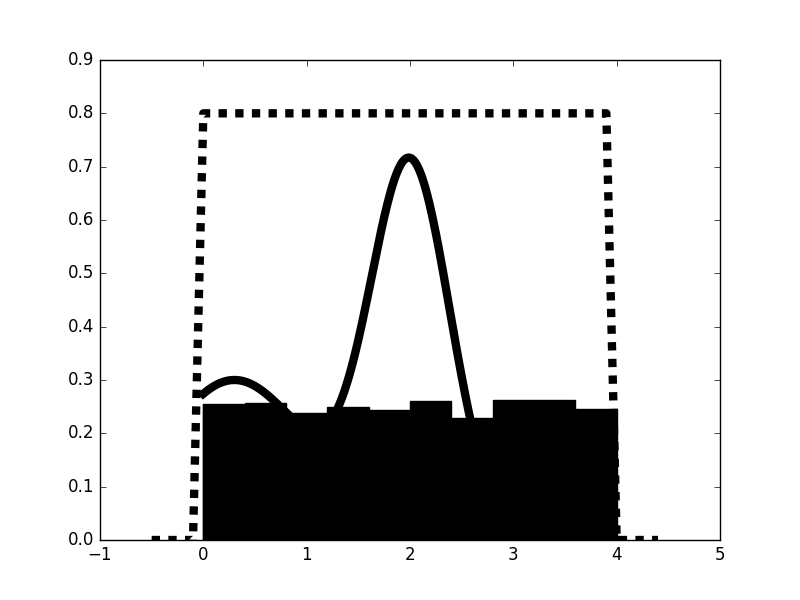
\includegraphics[height=6cm]{stat_mcmc_02.png}

Altta Örnekleme ve Öneme Göre Tekrar Örnekleme (Sampling İmportance Resampling)
metotu için örnek kod,

\begin{minted}[fontsize=\footnotesize]{python}
def p(x): return 0.3*exp(-(x-0.3)**2) + 0.7* exp(-(x-2.)**2/0.3) 

def q(x): return 4.0

def sir(n):    
    sample1 = np.zeros(n)
    w = np.zeros(n)
    sample2 = np.zeros(n)    
    sample1 = np.random.rand(n)*4
    w = p(sample1)/q(sample1)
    w /= sum(w)
    cumw = zeros(len(w))
    cumw[0] = w[0]
    for i in range(1,len(w)): cumw[i] = cumw[i-1]+w[i]
    u = np.random.rand(n)
    index = 0
    for i in range(n):
        indices = where(u<cumw[i])
        sample2[index:index+size(indices)] = sample1[i]
        index += size(indices)
        u[indices]=2
    return sample2

x = np.arange(0,4,0.01)
x2 = np.arange(-0.5,4.5,0.1)
realdata = 0.3*np.exp(-(x-0.3)**2) + 0.7* np.exp(-(x-2.)**2/0.3) 
box = np.ones(len(x2))*0.8
box[:5] = 0
box[-5:] = 0
plt.plot(x,realdata,'k',lw=6)
plt.plot(x2,box,'k--',lw=6)
plt.savefig('stat_mcmc_03.png')
\end{minted}

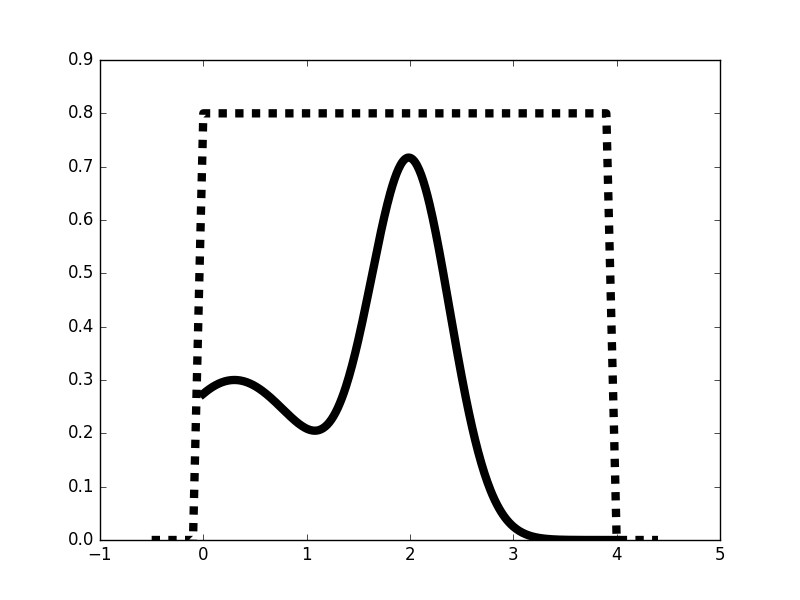
\includegraphics[height=6cm]{stat_mcmc_03.png}

MCMC

Yine $p(x)$'den örnekleme yapılamadığı durum, bu sefer $p(x)$ yerine onu
yaklaşıksal olarak temsil eden bir $\pi(x)$'i elde etmekle uğraşılıyor. Bu
$\pi(x)$ işe bir Markov Zincirinin (Markov Chain -yine MC harfleri!-) durağan
dağılımı olarak hayal ediliyor.

Markov Zinciri teorisinde bir geçiş matrisi, yan Markov Zincirinin kendisi
verilir, ve durağan dağılımın hesaplanması istenir. MCMC problemlerinde
ise, yani Monte Carlo entegralı için Markov Zinciri kullanıldığı durumlarda
elimizde bir $\pi(x)$ dağılımı vardır ve bir Markov Zinciri oluşturmamız
gerekir. Nihai dağılımı biliriz, ve bu dağılıma ``giden'' geçişleri
üretiriz. Bu geçişleri öyle ayarlayabiliriz ki üretilen rasgele sayılar
hedef dağılımından geliyormuş gibi olur. 

Geçişleri üretmek için literatürde bir çok teknik vardır.  Önemsel
Örnekleme (Importance Sampling), Örnekleme ve Öneme Göre Tekrar Örnekleme
(Sampling İmportance Resampling), Metropolis-Hastings, Gibbs Örneklemesi
gibi teknikleri vardır, ve detayları değişik olsa da hepsi de MCMC
kategorisine girer, ve yapmaya çalıştıkları $\pi(x)$'e giderken bir şekilde
bir geçişleri, zinciri ortaya çıkartmak ve bu geçişleri entegral hesabında
kullanmaktır.

Üstteki tekniklerden en yaygın kullanılanı Metropolis-Hastings
algoritmasıdır. 

Şunu vurgulamak önemli, geçişleri üretmek, ``bir tür sanal Markov Matrisi''
yaratmaktır aslında. Ve her MCMC algoritması bunu farklı şekillerde
yapabilir; mesela MH daha basit başka bir dağılım ile ana dağılım arasında
sürekli karşılaştırmalar yapar, belli aralıklarda geçiş yapar, diğerlerinde
yapmaz, ve bunun bir yan etkisi olarak ortaya bir Markov Zinciri çıkartmış
/ onu kullanmış olur. O geçişlerin bir Markov Zinciri'ne eşdeğer olduğunun
matematiksel olarak ispatı da vardır.

Not: Bu alandaki makalelerde bir dağılımın ``belli bir çarpımsal sabite
kadar'' bilindiği (known up to a multiplicative constant) söylenir. Bu söz
aslında şu anlama gelir. Mesela ayrıksal bir dağılımımız var, ama bu
dağılımın kendisini, şu halini biliyoruz

\verb![ 4.3  2.   8.4  8.7  1.8]!

Bu bir dağılım değil, çünkü öğelerin toplamı 1 değil. Onu bir dağılım
haline çevirmek için, tüm öğeleri toplamak ve bu vektördeki tüm sayıları bu
toplam ile bölmek gerekir. Toplam 25.2, bölersek

\verb![ 0.17063492  0.07936508  0.33333333  0.3452381   0.07142857]!

İlk vektör ``belli bir çarpımsal sabite kadar'' bilinen dağılım, çarpımsal
sabit 25.2. Esas dağılım ikinci vektör. 

Peki niye bu sözü söyleyenler toplamı hesaplayıp gerçek dağılımı
hesaplamıyorlar? Sebep performans. Bazen ayrıksal dağılım o kadar yüksek
boyutlu, fazla öğe içeren bir halde oluyor ki, performans açısından bu
basit toplam hesabını yapmak bile çok pahalı oluyor. İşte MCMC metotlarının
bir güzel tarafı daha burada, dağılımın kendisi olmasa bile belli bir
çarpımsal sabite kadar bilinen versiyonları ile gayet rahat bir şekilde
işliyorlar.

Metropolis-Hastings

\begin{minted}[fontsize=\footnotesize]{python}
def p(x):
    mu1 = 3; mu2 = 10
    v1 = 10; v2 = 3
    return 0.3*np.exp(-(x-mu1)**2/v1) + 0.7* np.exp(-(x-mu2)**2/v2)

def q(x):
    mu = 5; sigma = 10
    return np.exp(-(x-mu)**2/(sigma**2))

stepsize = 0.5
x = np.arange(-10,20,stepsize)
px = np.zeros(x.shape)
for i in range(len(x)): px[i] = p(x[i])
N = 5000

# independence chain
u = np.random.rand(N)
mu = 5
sigma = 10
y = np.zeros(N)
y[0] = np.random.normal(mu,sigma)
for i in range(N-1):
    ynew = np.random.normal(mu,sigma)
    alpha = min(1,p(ynew)*q(y[i])/(p(y[i])*q(ynew)))
    if u[i] < alpha:
        y[i+1] = ynew
    else:
        y[i+1] = y[i]

# random walk chain
u2 = np.random.rand(N)
sigma = 10
y2 = np.zeros(N)
y2[0] = np.random.normal(0,sigma)
for i in range(N-1):
    y2new = y2[i] + np.random.normal(0,sigma)
    alpha = min(1,p(y2new)/p(y2[i]))
    if u2[i] < alpha:
        y2[i+1] = y2new
    else:
        y2[i+1] = y2[i]

plt.figure(1)
nbins = 30
plt.hist(y, bins = x)
plt.plot(x, px*N/np.sum(px), color='r', linewidth=2)

plt.savefig('stat_mcmc_01.png')
\end{minted}

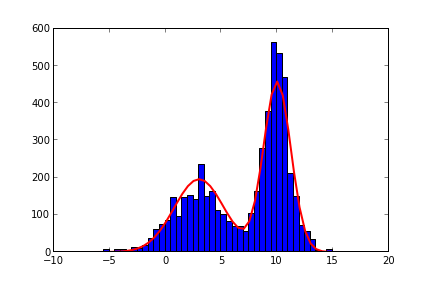
\includegraphics[height=6cm]{stat_mcmc_01.png}

Gibbs Örneklemesi

Bu örnekleme metodu Metropolis yönteminin bir versiyonu olarak kabul
edilir, Metropolis yöntemlerinde bir teklif (proposal) dağılımı $Q$ vardır,
ve bu dağılımın örneklenmek istenen $P$ ile ilişkisine göre zar atılıp elde
edilen yeni nokta kabul edilir, ya da kenara atılır. Gibbs ile de bir $Q$
vardır, ama bir cinlik yapılmıştır, $Q$ için $P$'nin kendisi, daha doğrusu
onun koşullu dağılım hali kullanılır. Bu koşullu dağılım her $i$ için
$P(x_i|\{x_j\}_{j \ne i}$, burada $x_i$ çok boyutlu $x$'in bir öğesidir,
$\{x_j\}_{j \ne i}$ işe $i$ olmayan diğer tüm öğelerdir. Yani $i$ {\em
  olmayan} her değişken koşulunda $i$ örneklenir. Bu kullanımın Metropolis
yöntemi ile aynı olduğu ispatlanmıştır. Koşullu dağılımın kullanılmasının
ana sebebi ise çok boyutlu $P$ zor bir dağılım olsa bile çoğunlukla onun
koşullu ve tek boyutlu dağılımının rahatça örneklenebilir halde olmasıdır.

Algoritma şöyle; Rasgele bir başlangıç noktasından başlanır, ve biri harici
tüm değişkenler sabit tutulup sabit olmayan değişken örneklenir. Bu işlem
sürekli uygulanır, bu yapılınca sanki örneklenen dağılımın en olası yerleri
gezilmiş olur. 

Mesela 2 boyutta, bir $x^{(t)}$ noktasından başladığımızı farzedelim,
$P(x_1|x_2)$ dağılımından bir $x_1$ örneklenir, (b) şeklinde koşullu
dağılımın tek boyutlu bir Gaussian olduğunu görüyoruz (çünkü ana dağılım
iki boyutlu Gaussian), bu tek boyutlu dağılımdan bir örneklem alınıyor,
doğal olarak o tek boyutlu dağılımın tepe noktasının altına yakın bir
yerden.

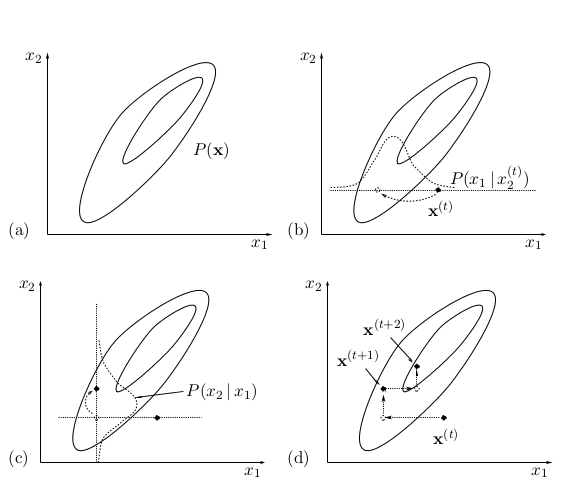
\includegraphics[height=8cm]{gibbs.png}

Sonra bu nokta sabitleniyor (yani yeni bir koşullu dağılım yaratılıyor, ve
örneklenen $x_1$ şimdi sağ tarafta), yani $P(x_2|x_1)$ dağılımından. Bu
bizi $x^{(t+1)}$ konumuna (state) götürüyor, bu böyle devam ediyor. $K$
değişken (boyutundaki) içeren bir sistemde, genel formüller şöyle,

$$ x_1^{(t+1)} \sim P(x_1 | x_2^{t},x_3^{t},..,x_K^{t}) $$ 

$$ x_2^{(t+1)} \sim P(x_2 | x_1^{t},x_3^{t},..,x_K^{t}) $$ 

$$ x_3^{(t+1)} \sim P(x_3 | x_1^{t},x_2^{t},..,x_K^{t}) $$ 

vs..

Monte Carlo ile $pi$ Hesabı

Yaklaşık olarak $\pi$'yi nasıl hesaplarız? İçinde $\pi$ olan hangi formülü
biliyoruz? Çember alanı formülü. Bunu nasıl kullanabiliriz. Yarıçapı $r$
olan bir çember düşünelim, ve bu çember bir kare içinde olsun, yani karenin
kenarları $2r$,

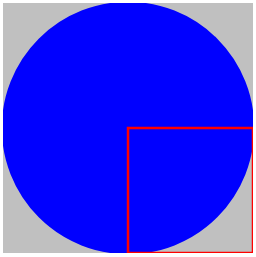
\includegraphics[width=10em]{stat_mcmc_05.png}

Bu durumda kırmızıyla işaretli bölgenin alanı $r^2$. Mavi çemberin alanı
ise $\pi r^2$, çemberin kırmızı bölge içine düşen kısmi $\pi r^2 / 4$. O
zaman ufak karenin oradaki çember kısminin alanına olan oranı
$p = \frac{\pi r^2}{4}$ olur. O zaman, eğer iki boyutlu birörnek bir
dağılımdan (yani üstteki karenin içine düşecek sayılar) örneklem alırsak,
bu her sayı için çember içine mi düşüyor, dışına mı düşüyor hesabı kolay,
$x,y$ sayısı için $x^2+y^2 < r^2$ ise çember içinde, değilse dışında. İçeri
düşen sayıların oranını $p$ kabul ederiz, bu sayıyı 4 ile çarpınca yaklaşık
$\pi$ elde edilir.

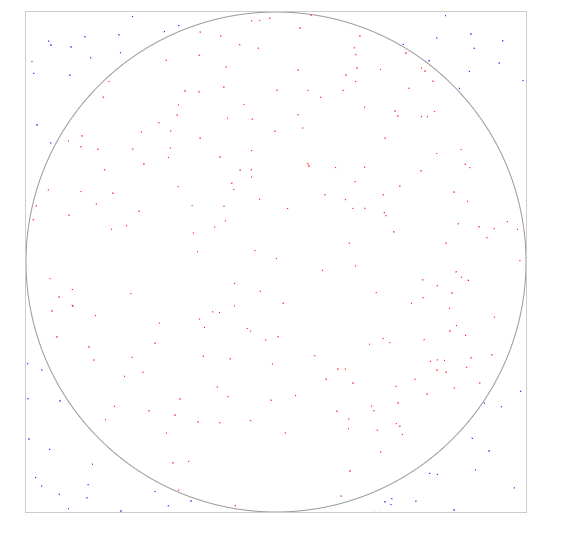
\includegraphics[width=15em]{stat_mcmc_04.png}

\begin{minted}[fontsize=\footnotesize]{python}
import random

NB_POINTS = 10**4
LENGTH = 10**5
CENTER = [LENGTH/2,LENGTH/2]

def in_circle(point):
    x,y = point
    center_x, center_y = CENTER
    radius = LENGTH/2
    return (x - center_x)**2. + (y - center_y)**2. < radius**2.

def compute_pi(nb_it):
    inside_count = sum(1.0 for _ in range(nb_it) if \
        in_circle( (random.randint(1,LENGTH),random.randint(1,LENGTH)) ) )
    return (inside_count / nb_it) * 4.

if __name__ == "__main__":
    print u'yaklaşık', compute_pi(NB_POINTS), u'gerçek', np.pi
\end{minted}

\begin{verbatim}
yaklaşık 3.1432 gerçek 3.14159265359
\end{verbatim}

Kaynaklar

[1] Marsland, {\em Algorithmic Machine Learning}

[2] MacKay, {\em Information Theory, Inference and Learning Algorithms}

[3] Turner, {\em An Introduction to Particle Filtering}, \url{http://www.lancaster.ac.uk/pg/turnerl/PartileFiltering.pdf}

\end{document}
